\usetikzlibrary{arrows.meta,calc,matrix,shapes}
\providecommand{\computer}{%
    
\includegraphics[width=1cm]{../common/Noun_project_216.pdf}
}
\providecommand{\switch}{%
    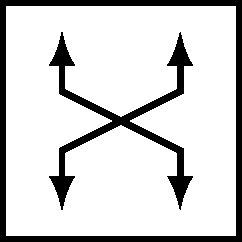
\includegraphics[width=0.9cm]{../common/fig-switch.pdf}
}
\providecommand{\router}{%
    
\includegraphics[width=0.9cm]{../common/fig-router.pdf}
}

\begin{frame}{spanning tree}
    \begin{itemize}
    \item given a general network, only activate subset of links
    \item \ldots such that network is tree
        \begin{itemize}
        \item that is only one path between each node
        \end{itemize}
    \vspace{.5cm}
    \item allows us to do flooding strategy
    \item makes simple MAC learning/broadcast just work
    \end{itemize}
\end{frame}

\begin{frame}{centralized spanning tree?}
    \begin{itemize}
    \item one algorithm you might learn in DSA2:
    \vspace{.5cm}
    \item mark one node called \textit{the root} as `in the tree'
    \item repeatedly: 
        \begin{itemize}
        \item add the `\myemph<2>{first}' link that goes to a node not in the tree
        \item mark newly connected node as `in the tree'
        \end{itemize}
    \vspace{.5cm}
    \item result = spanning tree
    \end{itemize}
\end{frame}

\begin{frame}{a careful ordering}
    \begin{itemize}
    \item algorithm works with any idea of which link/node is first
    \vspace{.5cm}
    \item we'll choose a particular ordering (for reasons you'll see later)
    \vspace{.5cm}
    \item first node one with earliest `name'
    \item links closer to the root before further links
    \item links from nodes with earlier names before later ones
    \end{itemize}
\end{frame}

\begin{frame}[fragile]{spanning tree example}
\begin{tikzpicture}
\tikzset{
    computer/.style={inner sep=0mm,outer sep=0mm,execute at begin node={\computer}},
    switch/.style={inner sep=0mm,outer sep=0mm,execute at begin node={\switch}},
    port/.style={pos=0.95,fill=white,circle,draw,inner sep=0mm},
    port beginning/.style={pos=0.05,fill=white,circle,draw,inner sep=0mm},
    route table/.style={
        matrix of nodes,ampersand replacement=\&,
        column 1/.style={nodes={draw,thick,text width=2.5cm,font=\tiny\tt,text depth=0mm,minimum height=0.5cm,inner sep=1mm}},
        column 2/.style={nodes={draw,thick,text width=.5cm,font=\small\tt,text depth=0mm,minimum height=0.5cm,inner sep=1mm}},
        row 1/.style={nodes={draw=none,font=\small}},
    },
    mac label/.style={
        draw,fill=white,inner sep=1mm,font=\tiny\tt,
    },
    tn/.style={draw,dotted,circle,very thick},
    real at/.style={alt=<#1->{solid},alt=<#1>{fill=red!10}},
    connect maybe/.style={draw,very thick,dotted,Latex-Latex},
    actual at/.style={alt=<#1->{draw=red,solid},alt=<#1>{draw,solid}},
    consider at/.style={alt=<#1>{draw=red}},
}
\node[tn,real at=1] (A) at (0, 0) {A};
\node[tn,real at=3] (B) at (5, -1) {B};
\node[tn,real at=4] (C) at (-5, -1) {C};
\node[tn,real at=6] (D) at (7, -3) {D};
\node[tn,real at=7] (E) at (1, -5) {E};
\node[tn,real at=8] (F) at (-7, -4) {F};
\draw[connect maybe,consider at=2,actual at=3] (A) -- (B)
    node[midway,sloped,above,visible on=<2>] {first priority};
\draw[connect maybe,consider at=2,actual at=4] (A) -- (C)
    node[midway,sloped,above,visible on=<2>] {second priority};
\draw[connect maybe,consider at=5] (B) -- (C)
    node[midway,sloped,below,visible on=<5>] {no new nodes};
\draw[connect maybe,actual at=6,consider at=5] (B) -- (D)
    node[midway,below left,visible on=<5>] {first priority};
\draw[connect maybe,actual at=7,consider at=5] (C) -- (F)
    node[midway,below right,visible on=<5>] {second priority};
\draw[connect maybe,actual at=8] (D) -- (E);
\draw[connect maybe] (E) -- (F);
\end{tikzpicture}
\end{frame}



\begin{frame}{distributing the algorithm}
\end{frame}
